\section{Ilham Muhammad Ariq D4TI2C 1174087}
\subsection{Keterampilan Pemrograman}
\begin{enumerate}
    \item Buatlah  fungsi  (file  terpisah/library  dengan  nama  \verb|NPM_csv.py|)  untuk  membuka file csv dengan lib csv mode list.
    
    \lstinputlisting[firstline=8, lastline=14]{src/4/1174087/Praktek/1174087_csv.py}

    \item Buatlah  fungsi  (file  terpisah/library  dengan  nama  \verb|NPM_csv.py|)  untuk  membuka file csv dengan lib csv mode dictionary.
   	
   	\lstinputlisting[firstline=16, lastline=20]{src/4/1174087/Praktek/1174087_csv.py}

	\item Buatlah fungsi (file terpisah/library dengan nama \verb|NPM_pandas.py|) untuk membuka file csv dengan lib pandas mode list.
	
	\lstinputlisting[firstline=7, lastline=11]{src/4/1174087/Praktek/1174087_pandas.py}
		
	\item Buatlah fungsi (file terpisah/library dengan nama \verb|NPM_pandas.py| untuk membuka file csv dengan lib pandas mode dictionary.

	\lstinputlisting[firstline=13, lastline=16]{src/4/1174087/Praktek/1174087_pandas.py}

	\item Buat fungsi baru di \verb|NPM_pandas.py| untuk mengubah format tanggal menjadi standar dataframe.

	\lstinputlisting[firstline=25, lastline=27]{src/4/1174087/Praktek/1174087_pandas.py}

	\item Buat fungsi baru di \verb|NPM_pandas.py| untuk mengubah index kolom.
	
	\lstinputlisting[firstline=29, lastline=32]{src/4/1174087/Praktek/1174087_pandas.py}
	
	\item Buat fungsi baru di \verb|NPM_pandas.py| untuk mengubah atribut atau nama kolom.
	
	\lstinputlisting[firstline=34, lastline=37]{src/4/1174087/Praktek/1174087_pandas.py}
	
	\item Buat program main.py yang menggunakan library \verb|NPM_csv.py| yang membuat dan membaca file csv.
	
	\lstinputlisting[firstline=8, lastline=15]{src/4/1174087/Praktek/main.py}
	
	\item Buat program main2.py yang menggunakan library \verb|NPM_pandas.py| yang membuat dan membaca file csv.

	\lstinputlisting[firstline=8, lastline=12]{src/4/1174087/Praktek/main2.py}
\end{enumerate} 

\subsection{Keterampilan Penanganan Error}

\begin{enumerate}
	\item Tuliskan peringatan error yang didapat dari mengerjakan praktek ketiga ini,
dan jelaskan cara penanganan error tersebut. dan Buatlah satu fungsi yang
menggunakan gunakan try except untuk menanggulangi error tersebut.

	\lstinputlisting[firstline=7, lastline=16]{src/4/1174087/Praktek/error.py}
	
	\par NameError adalah exception yang terjadi saat kode melakukan eksekusi terhadap local name atau global name yang tidak terdefinisi. Misalnya saat menjumlahkan variable yang tidak didefinisikan, memanggil function yang tidak ada, dan lain-lain.
	
\end{enumerate}

\textbf{Screenshoot Kode Program Python}

\begin{figure}[H]
 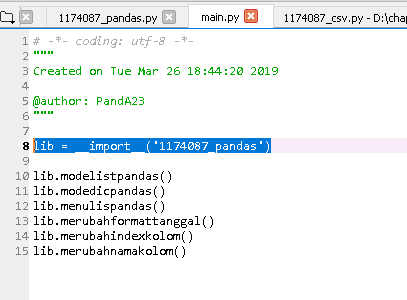
\includegraphics[width=5cm]{figures/4/1174087/Praktek/main.png}
 \centering
\end{figure}

\begin{figure}[H]
 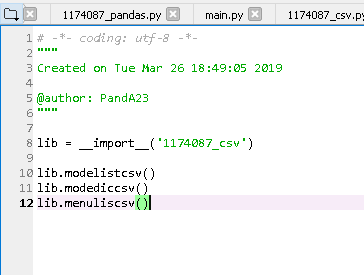
\includegraphics[width=5cm]{figures/4/1174087/Praktek/main2.png}
 \centering
\end{figure}

\begin{figure}[H]
 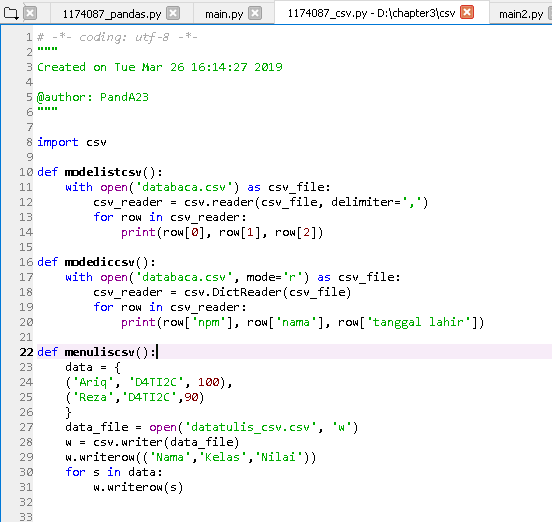
\includegraphics[width=5cm]{figures/4/1174087/Praktek/1174087_csv.png}
 \centering
\end{figure}

\begin{figure}[H]
 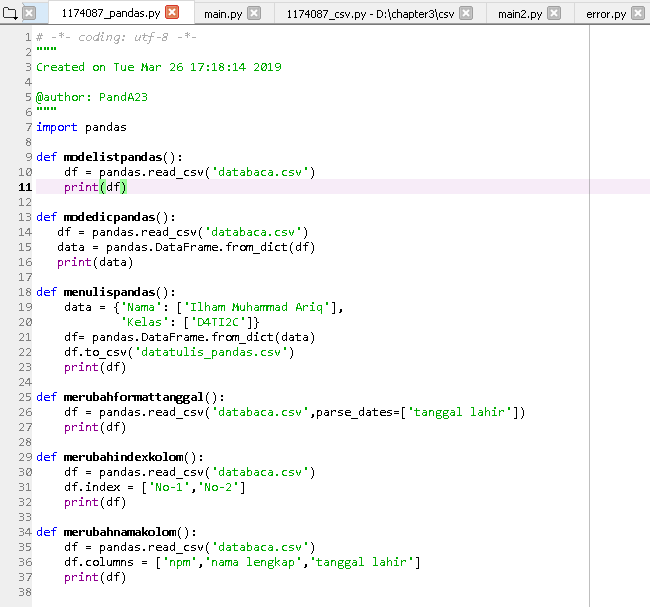
\includegraphics[width=5cm]{figures/4/1174087/Praktek/1174087_pandas.png}
 \centering
\end{figure}

\begin{figure}[H]
 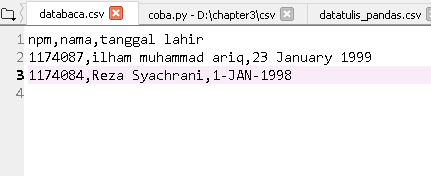
\includegraphics[width=5cm]{figures/4/1174087/Praktek/databaca.png}
 \centering
\end{figure}

\begin{figure}[H]
 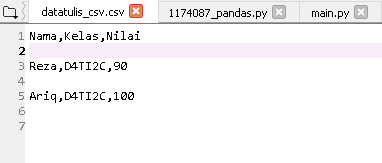
\includegraphics[width=5cm]{figures/4/1174087/Praktek/datatulis_csv.png}
 \centering
\end{figure}

\begin{figure}[H]
 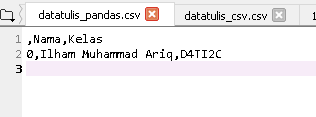
\includegraphics[width=5cm]{figures/4/1174087/Praktek/datatulis_pandas.png}
 \centering
\end{figure}

\begin{figure}[H]
 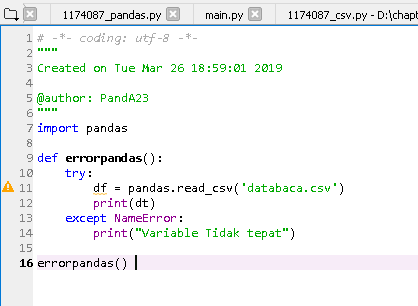
\includegraphics[width=5cm]{figures/4/1174087/Praktek/error.png}
 \centering
\end{figure}

%%%%%%%%%%%%%%%%%%%%%%%%%%%%%%%%%%%%%%%%%%%%%%%%%%%%%%%%%%%%%%%%%%%%%%%%%%%%%%%%%%%%%%%%%%%%%%%%%%%%%%%%%%%%%%%%%%%%%%
\section{Dini Permata Putri | 1174053}
\subsection{Keterampilan Pemrograman}
\begin{enumerate}
\item Buatlah  fungsi  (file  terpisah/library  dengan  nama  NPMcsv.py)  untuk  membuka file csv dengan lib csv mode list.


	\lstinputlisting[firstline=10, lastline=15]{src/4/1174053/Praktek/1174053csv.py}

	\item Buatlah  fungsi  (file  terpisah/library  dengan  nama  NPMcsv.py)  untuk  membuka file csv dengan lib csv mode dictionary.

	\lstinputlisting[firstline=17, lastline=22]{src/4/1174053/Praktek/1174053csv.py}

	\item Buatlah fungsi (file terpisah/library dengan nama NPMpandas.py) untuk membuka file csv dengan lib pandas mode list.

	\lstinputlisting[firstline=10, lastline=13]{src/4/1174053/Praktek/1174053pandas.py}

	\item Buatlah fungsi (file terpisah/library dengan nama NPMpandas.py) untuk membuka file csv dengan lib pandas mode dictionary.

	\lstinputlisting[firstline=10, lastline=13]{src/4/1174053/Praktek/1174053pandas.py}

	\item  Buat fungsi baru di NPMpandas.py untuk mengubah format tanggal menjadi standar dataframe.

	\lstinputlisting[firstline=15, lastline=19]{src/4/1174053/Praktek/1174053pandas.py}

	\item Buat fungsi baru di NPMpandas.py untuk mengubah index kolom.

	\lstinputlisting[firstline=21, lastline=24]{src/4/1174053/Praktek/1174053pandas.py}

	\item Buat fungsi baru di NPMpandas.py untuk mengubah atribut atau nama kolom.

	\lstinputlisting[firstline=26, lastline=30]{src/4/1174053/Praktek/1174053pandas.py}

	\item Buat program main.py yang menggunakan library NPMcsv.py yang membuat dan membaca file csv.

	\lstinputlisting[firstline=8, lastline=13]{src/4/1174053/Praktek/main.py}

	\item Buat program main2.py yang menggunakan library NPMpandas.py yang membuat dan membaca file csv.

	\lstinputlisting[firstline=8, lastline=13]{src/4/1174053/Praktek/main2.py}
\end{enumerate}

\subsection{Penanganan Error}
Peringatan error di praktek keempat ini, yaitu:
	\begin{itemize}
		\item Syntax Errors
		Syntax Error, adalah kesalahan yang disebabkan oleh kesalahan tata cara penulisan tanda baca, kesalahan pemakaian operator dan nilai. Kesalahan jenis ini akan dengan mudah dideteksi oleh kompiler maupun interpreter.

		\item Name Error
		NameError adalah exception yang terjadi saat kode melakukan eksekusi terhadap local name atau global name yang tidak terdefinisi. Misalnya saat menjumlahkan variable yang tidak didefinisikan, memanggil function yang tidak ada, dan lain-lain.

		\item Type Error
		TypeError adalah exception yang akan terjadi apabila pada saat dilakukannya eksekusi terhadap suatu operasi atau fungsi dengan type object yang tidak sesuai. Solusi dari error ini adalah mengkoversi varibelnya sesuai dengan tipe data yang akan digunakan.
	

	\item Fungsi yang menggunakan try except
	\lstinputlisting[firstline=55, lastline=67]{src/4/1174053/Praktek/1174053.py}
\end{itemize}